\documentclass[border=10pt]{standalone}
\usepackage[svgnames]{xcolor}
\usepackage{amsmath}
\usepackage{pgfplots}
\pgfplotsset{compat=newest}
\usepackage[sfdefault]{FiraSans}
\usepackage{FiraMono}
\renewcommand*\familydefault{\sfdefault}
\begin{document}
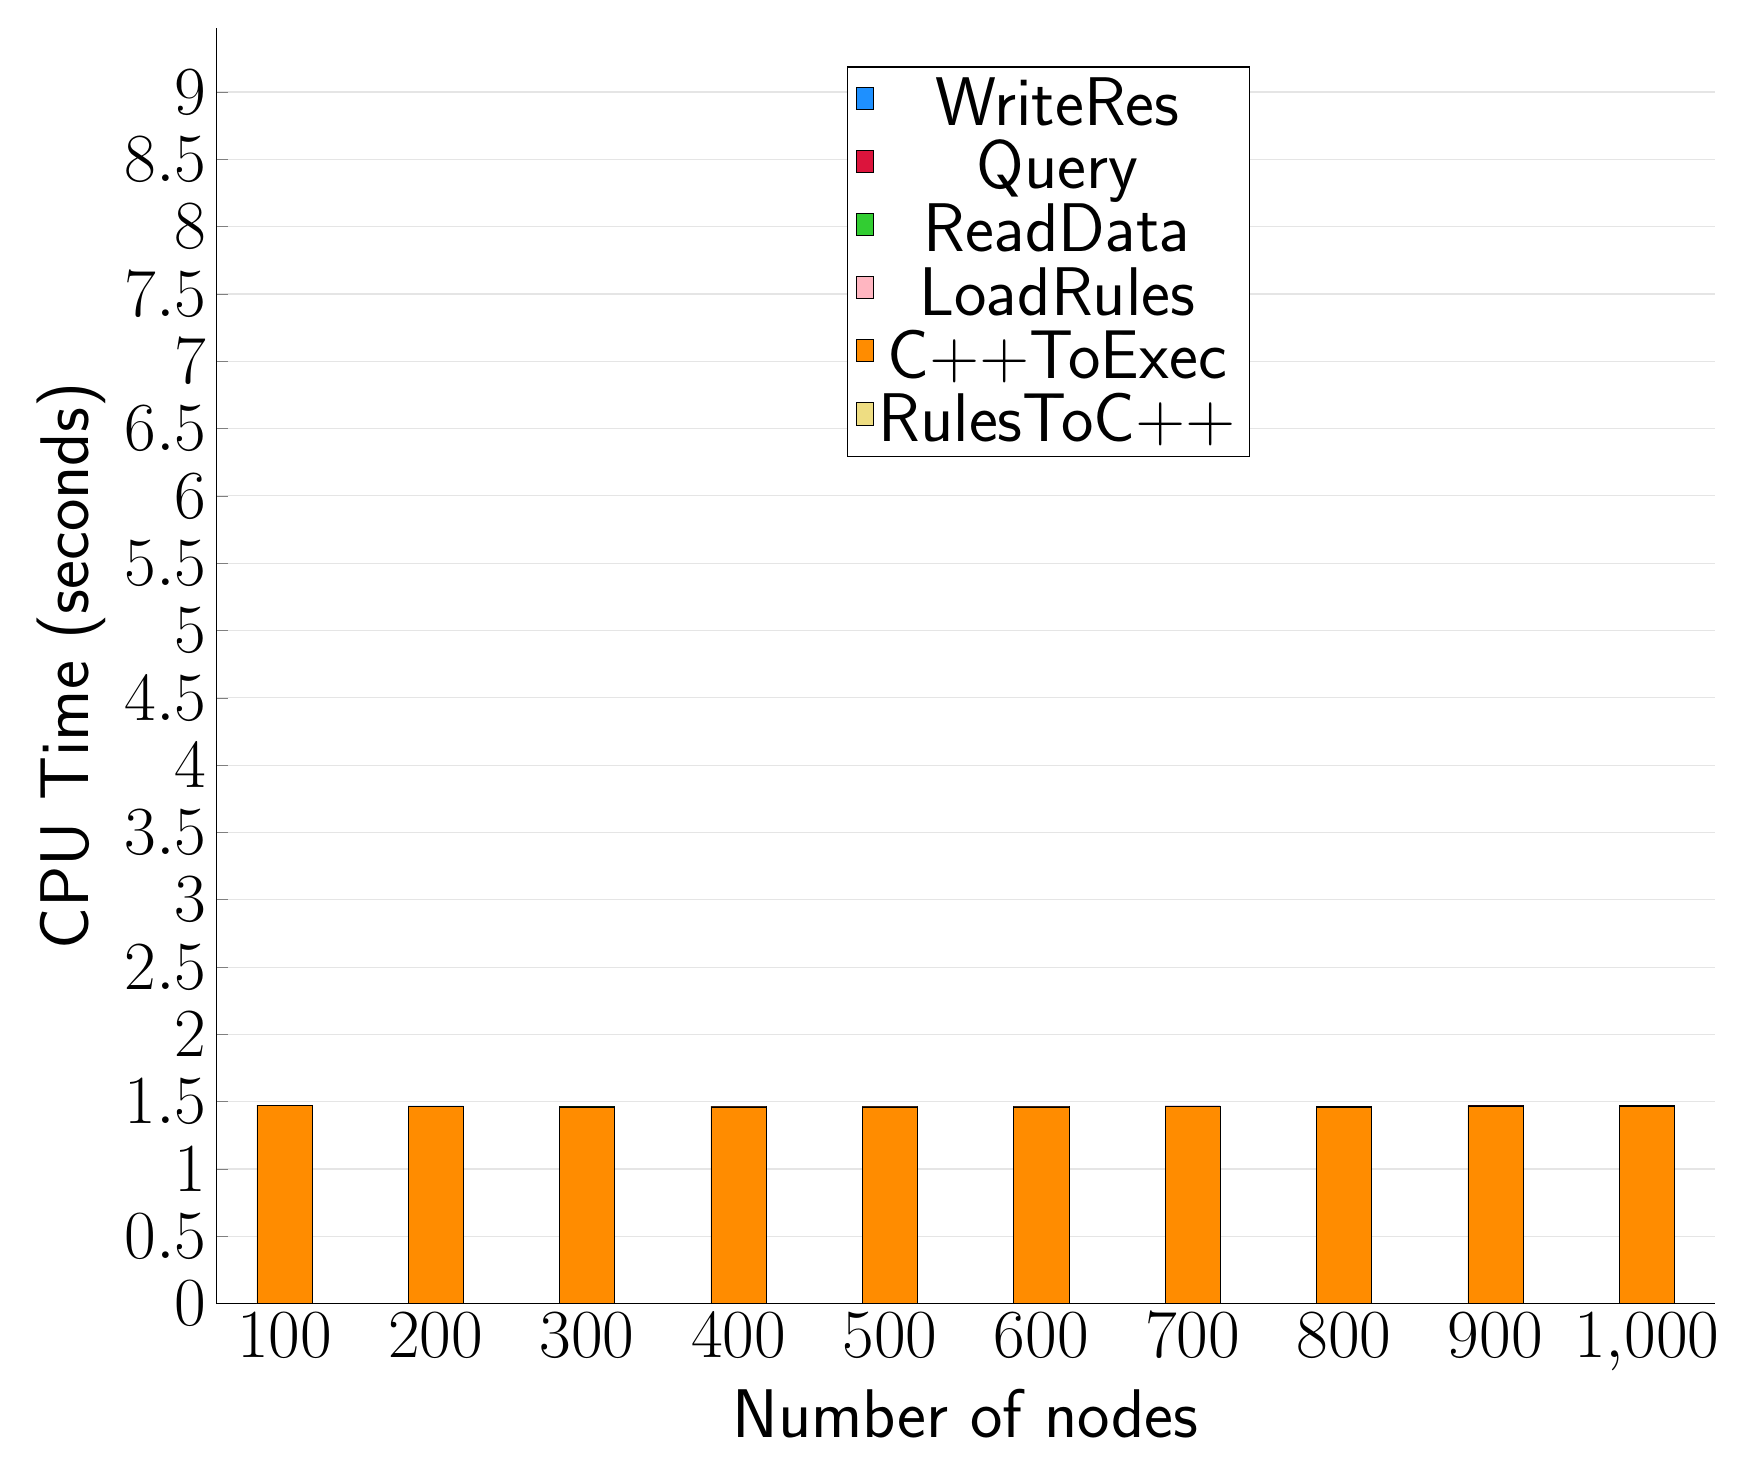
\begin{tikzpicture}
\begin{axis}[
   ybar stacked,
   width=1.7\textwidth,
   bar width=0.7cm,
   ymajorgrids, tick align=inside,
   major grid style={draw=gray!20},
   xtick=data,
   ymin=0, ymax=9.474,
   axis x line*=bottom,
   axis y line*=left,
   enlarge x limits=0.05,
   legend style={
       at={(0.69, 0.97)},
       anchor=north east,
       legend columns=1,
       font=\Huge,
   },
   ylabel={CPU Time (seconds)},
   xlabel={Number of nodes},
   label style={font=\Huge},
   tick label style={font=\Huge},
]
\addlegendimage{fill=DodgerBlue, draw=black, line width=0.2pt}
\addlegendentry{WriteRes}
\addlegendimage{fill=Crimson, draw=black, line width=0.2pt}
\addlegendentry{Query}
\addlegendimage{fill=LimeGreen, draw=black, line width=0.2pt}
\addlegendentry{ReadData}
\addlegendimage{fill=LightPink, draw=black, line width=0.2pt}
\addlegendentry{LoadRules}
\addlegendimage{fill=DarkOrange, draw=black, line width=0.2pt}
\addlegendentry{C++ToExec}
\addlegendimage{fill=LightGoldenrod, draw=black, line width=0.2pt}
\addlegendentry{RulesToC++}
\addplot +[fill=LightGoldenrod, draw=black, line width=0.2pt] coordinates {
(100, 0.0)
(200, 0.0)
(300, 0.0)
(400, 0.0)
(500, 0.0)
(600, 0.0)
(700, 0.0)
(800, 0.0)
(900, 0.0)
(1000, 0.0)
};
\addplot +[fill=DarkOrange, draw=black, line width=0.2pt] coordinates {
(100, 1.472)
(200, 1.4659999999999997)
(300, 1.46)
(400, 1.462)
(500, 1.462)
(600, 1.462)
(700, 1.464)
(800, 1.46)
(900, 1.464)
(1000, 1.466)
};
\addplot +[fill=LightPink, draw=black, line width=0.2pt] coordinates {
(100, 0.000148)
(200, 0.00015560000000000001)
(300, 0.0001446)
(400, 0.0001552)
(500, 0.0001496)
(600, 0.0001578)
(700, 0.00015940000000000003)
(800, 0.00016)
(900, 0.00015120000000000002)
(1000, 0.00015599999999999997)
};
\addplot +[fill=LimeGreen, draw=black, line width=0.2pt] coordinates {
(100, 0.0008122000000000001)
(200, 0.0012168)
(300, 0.0015872)
(400, 0.0019682)
(500, 0.0022366)
(600, 0.0027367999999999997)
(700, 0.0028764)
(800, 0.0033772000000000003)
(900, 0.0037278)
(1000, 0.004085)
};
\addplot +[fill=Crimson, draw=black, line width=0.2pt] coordinates {
(100, 0.00017680000000000001)
(200, 0.00035480000000000006)
(300, 0.0005342000000000001)
(400, 0.000691)
(500, 0.0008392)
(600, 0.0009948)
(700, 0.0011196000000000001)
(800, 0.0012502)
(900, 0.0013808000000000002)
(1000, 0.0016764000000000002)
};
\addplot +[fill=DodgerBlue, draw=black, line width=0.2pt] coordinates {
(100, 0.0005013999999999999)
(200, 0.0005054)
(300, 0.0006558)
(400, 0.0007289999999999999)
(500, 0.000735)
(600, 0.0008135999999999999)
(700, 0.0007827999999999999)
(800, 0.0009752000000000001)
(900, 0.0009464)
(1000, 0.0010745999999999998)
};
\end{axis}
\end{tikzpicture}

\end{document}
